% MEASUREMENT HARNESS --- not the submission.
%
% This exists to answer one question: how many pages is paper/body.tex? Every length decision was
% waiting on that number and it was UNKNOWN. It is deliberately in a subdirectory so that
% scripts/check_submission.py, which globs paper/*.tex non-recursively, does not mistake it for the
% real document. The real assembly happens in the jmlr skeleton outside this repository.
%
% The title block is placeholder text, anonymous by construction. Do not copy it anywhere.
%
%   /tmp/tectonic -X compile paper/harness/main.tex

\documentclass[wcp]{jmlr}

\usepackage{graphicx}
\graphicspath{{../../}}

\jmlrvolume{}
\jmlryear{2026}
\jmlrworkshop{Symmetry and Geometry in Neural Representations}

\title[Retained capacity decomposes forgetting]
      {What changes when a network forgets: a three-factor decomposition of retained
       manifold capacity}

\author{\Name{Anonymous Author} \Email{anon@example.invalid}}
\editors{Anonymous}

\begin{document}
\maketitle

% \typeout markers rather than a page-counting library: the count has to come from TeX itself,
% because a regex over the PDF bytes reads zero once the output uses compressed object streams,
% which is how the first attempt at this number silently returned 0 pages.
% Body of the NeurReps Extended Abstract --- a FRAGMENT, deliberately.
%
% No documentclass, no preamble, no document environment, no bibliography command. Paste the
% contents of this file into the jmlr skeleton after the title block, or \input it. Written this way
% because the skeleton holding the six-beat abstract outline is not in this repository, and a second
% main.tex would create a merge conflict with the real one instead of saving work.
%
% Needs from the skeleton's preamble: \usepackage{graphicx} and \graphicspath to reach figures/,
% or replace the paths in figures.tex. jmlr provides \floatconts.
% Companion files: figures.tex (the floats), references.bib (13 entries, 3 fields still to look up).
%
% Every number below is in docs/08-inventory.md against the artifact it is read from and the arm
% count it is computed over. Do not edit a number here without re-running
% `python scripts/make_inventory.py`, which verifies 25 of them against the exact sentence that
% quotes them and will fail if a sentence changes underneath its value.

\begin{abstract}
Catastrophic forgetting is normally measured as a loss of accuracy, which says how much was lost
and nothing about what changed in the representation. We measure forgetting as a change in
\emph{retained} manifold capacity --- the capacity of a representation for a specific past task's
labels --- which obeys an exact identity in three geometric factors and can therefore be attributed
without a model of what forgetting is. Sweeping feature-learning strength $\gamma_0$ over three
orders of magnitude in a 16-task stream, we find that forgetting is absent in the lazy regime and
reaches 69.7 times the estimator's own measurement noise in the rich regime, and that the channel
carrying it changes character along the way: the loss is mostly manifolds inflating relative to
their separation at intermediate richness and mostly a loss of alignment with the old task's labels
in the rich regime. One of the four task-similarity conditions does not forget but \emph{gains}
retained capacity, at every task position and every lag the design resolves, and the decomposition
shows why this is not forgetting with a sign flip: the gain is carried by alignment and dimension,
while the radius channel that dominates the losses is, in that condition, below resolution. Two
pre-registered predictions fail in sign rather than in magnitude --- the predicted crossing between
generic and task-specific capacity does not exist, and centers converge where we predicted they
would decorrelate --- and in both cases the geometry supports a more specific claim than the one we
registered.
\end{abstract}

\begin{keywords}
manifold capacity, representational geometry, continual learning, feature learning, catastrophic
forgetting, task similarity
\end{keywords}

\section{Introduction}

Forgetting is usually reported as a drop in accuracy on a past task. That measurement is decisive
about magnitude and silent about mechanism: two networks that forget equally may have done so
because their class manifolds inflated, because those manifolds spread into more dimensions, or
because the directions that once separated them stopped aligning with the task's labels. These are
different failures with different remedies, and an accuracy curve cannot distinguish them.

Manifold capacity \citep{chung2018classification,cohen2020separability} gives a currency in which
the distinction is expressible. We use the \emph{retained} capacity $\alpha(\cdot\,;y_j)$ ---
capacity for one specific past task's labels rather than for arbitrary dichotomies --- and the
exact three-factor identity of \citet{chou2026diagnosing},
%
\begin{equation}
\Delta \log \alpha
  = \underbrace{\Delta \log \Psi_{\mathrm{eff}}}_{\text{alignment with the labels}}
  + \underbrace{\Delta \log\!\left(1 + R_{\mathrm{eff}}^{-2}\right)}_{\text{manifold radius}}
  - \underbrace{\Delta \log D_{\mathrm{eff}}}_{\text{effective dimension}} .
  \label{eq:identity}
\end{equation}
%
Because \eqref{eq:identity} is an identity rather than a fit, an observed change in retained
capacity is \emph{attributed} rather than explained: the three terms sum to the whole with no
residual to argue about, and the question becomes which of them moved. Across 48{,}640 evaluations
the identity closes to $4.4\times10^{-16}$.

We ask how the attribution depends on feature-learning strength, and on how similar consecutive
tasks are. Both are pre-registered sweeps with kill criteria fixed in advance; the outcomes of all
nine registered hypotheses, including four that failed, are in Appendix~\ref{app:prereg}.

\section{Setup}

We train networks on a stream of 16 binary tasks and measure the geometry of a fixed set of class
manifolds at every task boundary, so that any past task's retained capacity can be read at the
boundary where it was learned and again at any later one. Richness is the feature-learning strength
$\gamma_0$ of \citet{graldi2025lazy}, swept over six levels from $0.03$ to $10$. Task similarity
follows the $2\times2$ design of \citet{hiratani2024disentangling}, which varies input-feature
similarity and readout similarity independently: \texttt{S-HH} (both high), \texttt{S-HL} (the same
stimuli under different rules, predicted catastrophic), \texttt{S-LH}, and \texttt{S-LL}. The
registered grid is 960 files at 40 per condition per richness; those 40 are 8 unique seeds
written five times --- \texttt{stream\_id} was stored in the filename and never read --- so
inference on the grid is at unique $n=8$, with arrangement and initialisation confounded.
New arms after the RNG fix are genuine $n=40$. A genuine-$n$ width arm at $\gamma_0=10$, a
crossed arrangement$\times$init run, and the $\gamma_0=30$ probe are appendix robustness; they
are not pooled with the registered grid. Channel reorganisation and the corner ordering
reproduce across three independent arrangements, so those results are not arrangement-specific.

\paragraph{Everything is denominated in a measured floor.}
Every magnitude we report is in units of the estimator's own Monte-Carlo dispersion, measured
directly at each richness level by re-measuring one fixed trained representation under several
measurement seeds \citep{chou2025beyond,chou2025glue}. This is what allows ``unchanged'' to be a
measurement rather than a small number. For $\alpha$ the dispersion is flat in $\gamma_0$
(CV 1.49--2.03\%, against 1.87\% registered), so magnitudes are comparable across the sweep; for
$R_{\mathrm{eff}}$ it is not flat, which matters for one gate and is recorded in the appendix.

\section{Forgetting decomposes, and the channel carrying it shifts with richness}

Measured for task~0 twelve task boundaries after it was learned, retained capacity is unchanged in
the lazy regime --- 0.2 floors at $\gamma_0 = 0.03$, which is nothing --- and falls by 69.7 floors
at $\gamma_0 = 10$ (Figure~\ref{fig:decomposition}a). Forgetting first becomes resolvable between
$\gamma_0 = 0.1$ and $0.3$ and then grows by two orders of magnitude.

Over the range where it is resolvable at all, the composition changes character. The alignment
channel grows from 0.08 to 0.45 of total motion while the radius channel falls from 0.39 to 0.11;
the dimension channel falls from 0.53 to 0.44 across the first step and is flat thereafter
(Figure~\ref{fig:decomposition}b). So from $\gamma_0 = 0.3$ onward the reorganisation is a straight
exchange between alignment and radius. \textbf{Lazy-regime and rich-regime forgetting are not the
same process at different intensities}: at intermediate richness capacity is lost mostly because
manifolds inflate relative to their separation, and in the rich regime mostly because the
representation's alignment with the old task's labels degrades.

Part of the radius channel is centers collapsing rather than manifolds inflating. Converting the
measured change in center correlation $\rho_c$ through a synthetic-manifold calibration, the
center-attributable share of the radius change rises from 0.05 to 0.44 through $\gamma_0 = 3$ and
then flattens --- the $\gamma_0 = 3 \to 10$ step is not resolved (bootstrap CI $[-0.038, +0.070]$),
so the reading is a steep rise followed by a plateau rather than a monotone climb.

\section{One corner gains capacity, and the decomposition says why that is not a sign flip}

The numbers above pool the three conditions that lose retained capacity. The fourth, \texttt{S-HH},
\emph{gains} it: $\Delta\log\alpha$ is positive at every richness, largest at $\gamma_0 = 1$ with
11.8 floors and falling to 6.2 by $\gamma_0 = 10$, with behavioural forgetting zero to within
measurement ($-0.0005$ to $+0.0001$). This is a property of that corner rather than a tendency
present elsewhere in weaker form: across 520 cells --- every combination of richness, condition,
width, task position and lag in the registered grid, plus the width arms and an out-of-range probe
--- \textbf{every resolvable gain is an \texttt{S-HH} cell}, and the largest gain anywhere outside
it reaches 0.74 floors, a third of the resolution gate.

\paragraph{It is backward transfer, not a privilege of the first task.}
All ten (task, lag) cells of the benign corner gain resolvably, at each of $\gamma_0 = 1$, 3 and 10
--- thirty cells with no exceptions. Since lag and task position are confounded by construction in
a stream of finite length, we read each from its own matched series and pool neither: at matched
lag~4 the gain is $+8.7$, $+12.6$ and $+12.8$ floors for tasks 0, 4 and 8 at $\gamma_0 = 10$, and
within task~0 it runs $+8.7$, $+9.0$, $+6.2$ and $+3.1$ floors at lags 4, 8, 12 and 15. If
anything the first task benefits least, and the gain weakens with elapsed time rather than
accumulating.

\paragraph{Two channels carry the gain; the third is too small to sign.}
In the three corners that forget, the radius term is large and well resolved for $\gamma_0 \geq 0.3$
--- 5.0 to 24.4 floors, reaching $-0.131$ to $-0.157$ at $\gamma_0 = 10$ --- so there the growth of
$R_{\mathrm{eff}}$ demonstrably works against retained capacity. In the corner that gains it is
\emph{not} resolved at any $\gamma_0 \geq 1$ as a single measurement: 1.9, 0.2 and 1.1 floors at $\gamma_0 = 1$, 3 and 10,
against the two-floor convention this paper applies everywhere else, and against the analysis's own
$3\sigma$ $R_{\mathrm{eff}}$ gate. The term's mean over the 8 unique seeds is 3.9 SEM from zero at
$\gamma_0 = 1$ and 2.5 at $\gamma_0 = 10$, so it is distinguishable as a population mean and not as a
single measurement --- the $3\sigma$ gate answers the second question and is not moved. We therefore
claim no sign for a typical arm, only a bound --- under 2 floors, where the three forgetting corners carry 11.7 to 14.1, so at
most a sixth of theirs. The two channels that are resolved both favour the gain: $+2.3$ floors
alignment and $+5.7$ dimension at $\gamma_0 = 10$, or as signed fractions of the net change
$+0.48$ utility and $+0.62$ dimension against $-0.11$ radius that the floor does not resolve, where
the pooled loss is $+0.45$, $+0.44$ and $+0.11$ with all three resolved. \textbf{Gain and loss are
not one process with two signs: the gain is carried by alignment and dimension, and the radius cost
that dominates the losses is absent from it to within resolution.} This is the argument for
decomposing rather than measuring magnitude: a magnitude-only account makes gain and loss the same
quantity with opposite signs, and cannot see that they differ in which channels carry them.

\paragraph{We do not locate the peak.}
At lag~12 the peak of the gain is sharply determined --- interpolating in $\log\gamma_0$ puts it at
1.23 with a paired-bootstrap interval of $[1.12, 1.35]$ at unique $n=8$, a sixth of a grid step. That precision
is real and beside the point, because the peak moves monotonically with lag: 2.86, 1.75, 1.23 and
0.96 at lags 4, 8, 12 and 15, nearly a full grid step end to end. There is no richness at which
backward transfer is strongest; there is one per lag, and the question is ill-posed without fixing
the lag. We report the shape --- rising from the lazy regime, peaking within the sampled range, and
decaying --- and claim no location.

\section{Both capacity measures rise, and two label-agnostic diagnostics disagree}

We predicted that generic capacity, for arbitrary dichotomies, would \emph{fall} with richness while
retained capacity rose, so that their product would peak at an interior $\gamma_0$. Generic capacity
rises instead, 0.3043 to 0.3750, resolvable at 11.3 floors; retained rises faster, 0.3129 to 1.3710,
a factor of 4.4, and exceeds generic at \emph{every} richness including the laziest ($+0.0086$),
with the gap widening monotonically to $+0.9960$. The object the prediction was built on does not
exist. The rise is not uniform: \texttt{S-LH} is the only condition whose generic capacity falls
($0.3038 \to 0.2898$), and \texttt{S-HL}, the predicted catastrophic corner, rises most (0.4507).

The sharper result is that correlations between these measures reverse sign depending on whether they
are computed across richness levels or within one, and that this is \emph{general} rather than a fact
about one pair. Over seven measures and all 28 pairs, 8 reverse. The mechanism is that richness moves
almost every measure monotonically, so a single common cause drags the between-level correlation
toward $\pm1$ while the within-level correlation reflects arm-to-arm variation at fixed richness ---
Simpson's paradox with richness as the confound, and in this design closer to the default than to a
discovery.

One instance is worth stating because both of its measures are label-agnostic and both are read as
proxies for representation quality. Generic capacity rises by 11.3 floors across the sweep while the
margin achieved by a refit linear readout on a random dichotomy --- the probe protocol of
\citet{johnston2023abstract} --- \emph{falls} over the same range ($0.0673$ at $\gamma_0 = 1$ to
$0.0531$ at $\gamma_0 = 10$), and yet within a fixed richness the two correlate positively ($+0.322$
at $\gamma_0 = 10$). This pair is not the strongest case: its between-level rank correlation is
$-0.429$ against a within-level mean of $+0.180$, weaker than all eight of the reversing pairs, and
six richness levels cannot carry a correlation of that size. \textbf{What generalises is the
mechanism, not a property of this pair} --- comparing representation-quality measures across a
hyperparameter that moves both of them can invert the conclusion drawn at fixed hyperparameter, which
is a more useful caution than the crossing would have been.

\section{Center geometry separates into two independent effects}

Both pre-registered predictions about center geometry fail. We predicted centers would
\emph{decorrelate} over a stream, following the progressive decorrelation reported in human
sequential practice by \citet{menghi2025similarity}; three of four conditions converge instead. We
predicted the largest center movement in the catastrophic corner \texttt{S-HL}; the largest is
\texttt{S-LH} ($+0.110$), twice \texttt{S-HL}'s magnitude ($-0.055$) and in the opposite direction.
All four conditions begin at the same place ($\rho_c = 0.391$--$0.392$), so the split is produced by
training and not by initialisation (Figure~\ref{fig:corners}a).

Read as a $2\times2$ rather than as a single ordering, the design separates cleanly: readout
similarity drives center \emph{convergence} ($+0.104$) and feature similarity drives center
\emph{decorrelation} ($-0.061$), with an interaction at the resolution limit ($+0.006$) and an
additive model predicting the held-out corner to within 0.012. Richness sets the gain on both
effects at a roughly constant ratio; the design sets the sign. And one corner does decorrelate:
\texttt{S-HL}, the same stimuli under different rules, progressively over the stream rather than at
its end, with the per-arm rank correlation between $\rho_c$ and block index negative on 8 of 8
unique seeds ($p=0.0078$, the floor of a two-sided sign test at $n=8$; 40 files are five copies of those seeds), median $-0.79$. That progressive form is what makes the correspondence with the human result
a correspondence rather than a coincidence of endpoints. The crossed run settles the sign and
qualifies the size: all 40 initialisations decline in each of its three arrangements, while the
magnitude runs from $-0.026$ to $-0.051$ across them, so what we claim is the ordering and not
$-0.055$ as a population value. The onset is bracketed by the registered grid --- absent at
$\gamma_0 = 3$ ($+0.003$, 4 of 8 unique, $p=1.0$) and present at $\gamma_0 = 10$ (8 of 8) --- a
factor of 3.3. A probe at $\gamma_0 = 5$, scored at eight arrangements against a rule written
before those arms existed, is negative in four of eight (95\% interval over arrangements
$[-0.023, +0.010]$), so it does not narrow that bracket.

\section{What the result survives}

\paragraph{Width.}
At genuine $n=40$, a $4\times$ change in load ($N = 150, 600$ at $\gamma_0 = 10$; $N=300$ is
the registered grid at unique $n=8$ and is not in this contrast) moves three-corner forgetting
by 0.62\% and the alignment share by 0.020. Two widths, not a located dependence. The one width
dependence worth reporting is internal to the two non-alignment channels --- the radius share falls
with width ($0.146 \to 0.098$) while dimension rises ($0.394 \to 0.463$), their sum moving far less
($0.540 \to 0.560$) --- so width moves the radius/dimension boundary and not the
alignment/non-alignment division.

\paragraph{Lag and task position.}
Both matter and they are confounded by construction, since long lags are available only to early
tasks. Measured separately, position is the larger effect: within task~0 forgetting grows
$1.29\times$ from lag 4 to 15, while at fixed lag~4 it grows $1.56\times$ from task 8 to task 0. The
\emph{composition} is insensitive to the choice --- shares agree to within 0.032 at every richness
between lag 12 and lag 4, against a richness-driven swing of 0.37 in the alignment share --- so the
main figure's cell determines the magnitude reported and not the mechanism.

\paragraph{What does not vary, and why the design is paired.}
Regressing per-arm forgetting on candidate sources at $\gamma_0 = 10$, the initialisation a run was
trained from explains none of it ($R^2 = 0.007$). Stream identity was stored in the filename and
never consumed, so the quoted stream $R^2 = 0.000$ is tautological on that grid. The crossed
arrangement$\times$init run measures stream $R^2 = 0.001$. What does explain forgetting are two
comparable sources --- how far the task sat
above the common asymptote when it was left, together with its elapsed lag ($0.589$), and which
corner the stream occupies ($0.523$) --- reaching $0.882$ together. We do not rank them; they
overlap through a corner-by-position interaction and the design was not built to separate them.

\section{Discussion}

Measuring forgetting in a currency that decomposes changes which questions are answerable. The
finding we would not have reached with an accuracy curve, or with a magnitude-only geometric
measure, is that the corner which gains retained capacity gains it through alignment and dimension,
while the radius channel that dominates the three corners that lose is, in that corner, bounded
below resolution. Backward transfer here is not forgetting with a sign flip; it is a different
composition of the same three channels, and only a decomposition can tell the two apart.

Two limits bound this. The stream is short and synthetic, so lag and task position cannot be fully
separated and we report them from matched series rather than pooling. And four of nine registered
predictions failed, three of them in sign --- a rate worth stating plainly, since in each case the
geometry supported a more specific claim than the registered one, and a reader has no way to tell
post-hoc specificity from pre-registered success unless the failures are listed. They are, in
Appendix~\ref{app:prereg}, alongside an appendix on the six families of error our own numbers had to
be corrected for. The count is a property of how carefully the record was kept --- the checks were
built as the work went --- not of how unusual the codebase is. One of them, found last, is a field
stored in a filename that was never read, so the files were correct and the $n$ was wrong.

\typeout{HARNESS BODYEND=\thepage}
% Figure floats for the NeurReps Extended Abstract.
%
% % Figure floats for the NeurReps Extended Abstract.
%
% % Figure floats for the NeurReps Extended Abstract.
%
% \input{figures} from the jmlr skeleton's body. Every float uses \floatconts, which the jmlr
% class provides, so captions sit above the graphic and \label lives inside the float.
%
% The \includegraphics filenames are the manifest names verbatim, hashes and arm counts included.
% They are ugly on purpose: the hash is the result set the figure was drawn from and the arm count
% is the n behind it, so a stale PDF cannot be swapped in without the filename changing. Do not
% rename them, and do not strip the hash to tidy the directory listing --- the correspondence to
% figures/MANIFEST.json is what makes the figure checkable, and scripts/check_submission.py
% verifies that every \includegraphics here names a file the manifest currently claims.
%
% Captions are the drafts in docs/07-writeup.md sections D and E, with citations attached.

\begin{figure}[t]
\floatconts
  {fig:decomposition}
  {\caption{\textbf{Forgetting decomposes exactly, and the channel that carries it shifts with
   richness.} Retained capacity for task~0 at lag~12, decomposed by the exact identity of
   \citet{chou2026diagnosing}. Pooled over the three conditions that lose capacity (24 unique seeds
   per $\gamma_0$; 120 files are five copies); \texttt{S-HH} is Figure~\ref{fig:benign}.
   \textbf{(a)}~Magnitude in noise floors, signed: 0.2 at $\gamma_0=0.03$ to 69.7 at $\gamma_0=10$.
   Grey band: $\pm 2$ floors.
   \textbf{(b)}~Channel shares, $|\mathrm{term}|/\sum|\mathrm{term}|$, drawn where the total clears
   the band. $\gamma_0=0.1$ hatched (margin inside the floor's uncertainty); $\gamma_0=0.3$ and
   above solid: utility $0.08\to0.45$, radius $0.39\to0.11$, dimension $0.53\to0.44$ then flat.
   \textbf{(c)}~Signed terms; utility negative on 100\% of arms for $\gamma_0\geq 1$.
   \textbf{(d)}~Center-collapse share of the radius channel, $0.05\to0.44$ through $\gamma_0=3$ then
   flat ($\gamma_0=3\to10$ step unresolved, CI $[-0.038,+0.070]$). Each bar gated at $3\times$ its
   own $R_{\mathrm{eff}}$ floor; coverage is not comparable across bars.
   Lag~12 exists only for task~0, the most-forgotten task --- the largest forgetting in the grid,
   not its average.}}
  {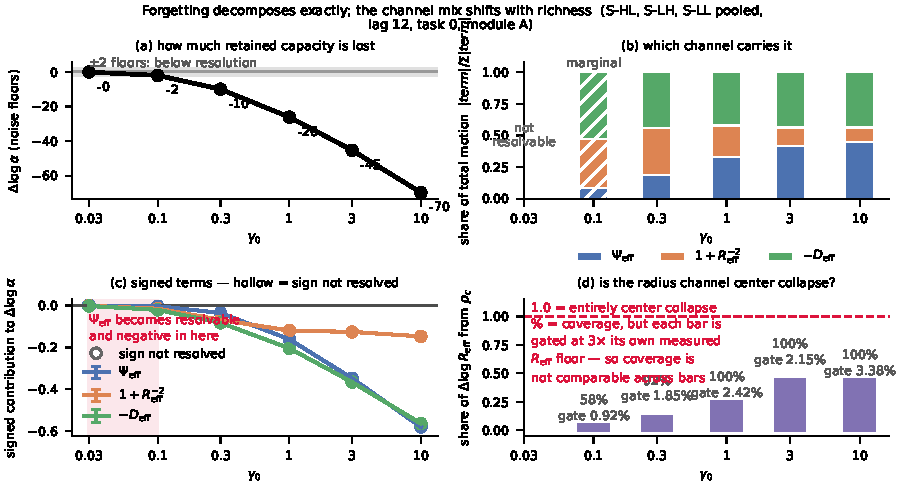
\includegraphics[width=\linewidth]
   {figures/fig2_gamma_sweep__forgetting__lag12__960arms__8dd793134c38.pdf}}
\end{figure}

\begin{figure}[t]
\floatconts
  {fig:corners}
  {\caption{\textbf{Center correlation moves in opposite directions across the similarity design,
   and the two axes act almost separately.}
   \textbf{(a)}~Signed $\rho_c$ at $\gamma_0=10$, design of \citet{hiratani2024disentangling}. All
   four corners start together ($\rho_c = 0.391$--$0.392$); three converge, \texttt{S-HL} (same
   stimuli, different rules) decorrelates.
   \textbf{(b)}~Grey band: lazy-arm drift ($\gamma_0=0.03$). \texttt{S-LL} never leaves it.
   \textbf{(c)}~\texttt{S-HL} decline is progressive, negative on 8 of 8 unique seeds
   ($p=0.0078$, the floor of a two-sided sign test at $n=8$; 40 files are copies), median Spearman
   $-0.79$.
   \textbf{(d)}~H1d and H6 fail in sign: three of four corners converge; largest $|\Delta\rho_c|$ is
   \texttt{S-LH}, twice \texttt{S-HL}.
   \textbf{(e)}~Readout $+0.104$, feature $-0.061$, interaction $+0.006$; additive error $0.012$.
   \textbf{(f)}~Both main effects survive a $4\times$ width change, ordering unchanged.}}
  {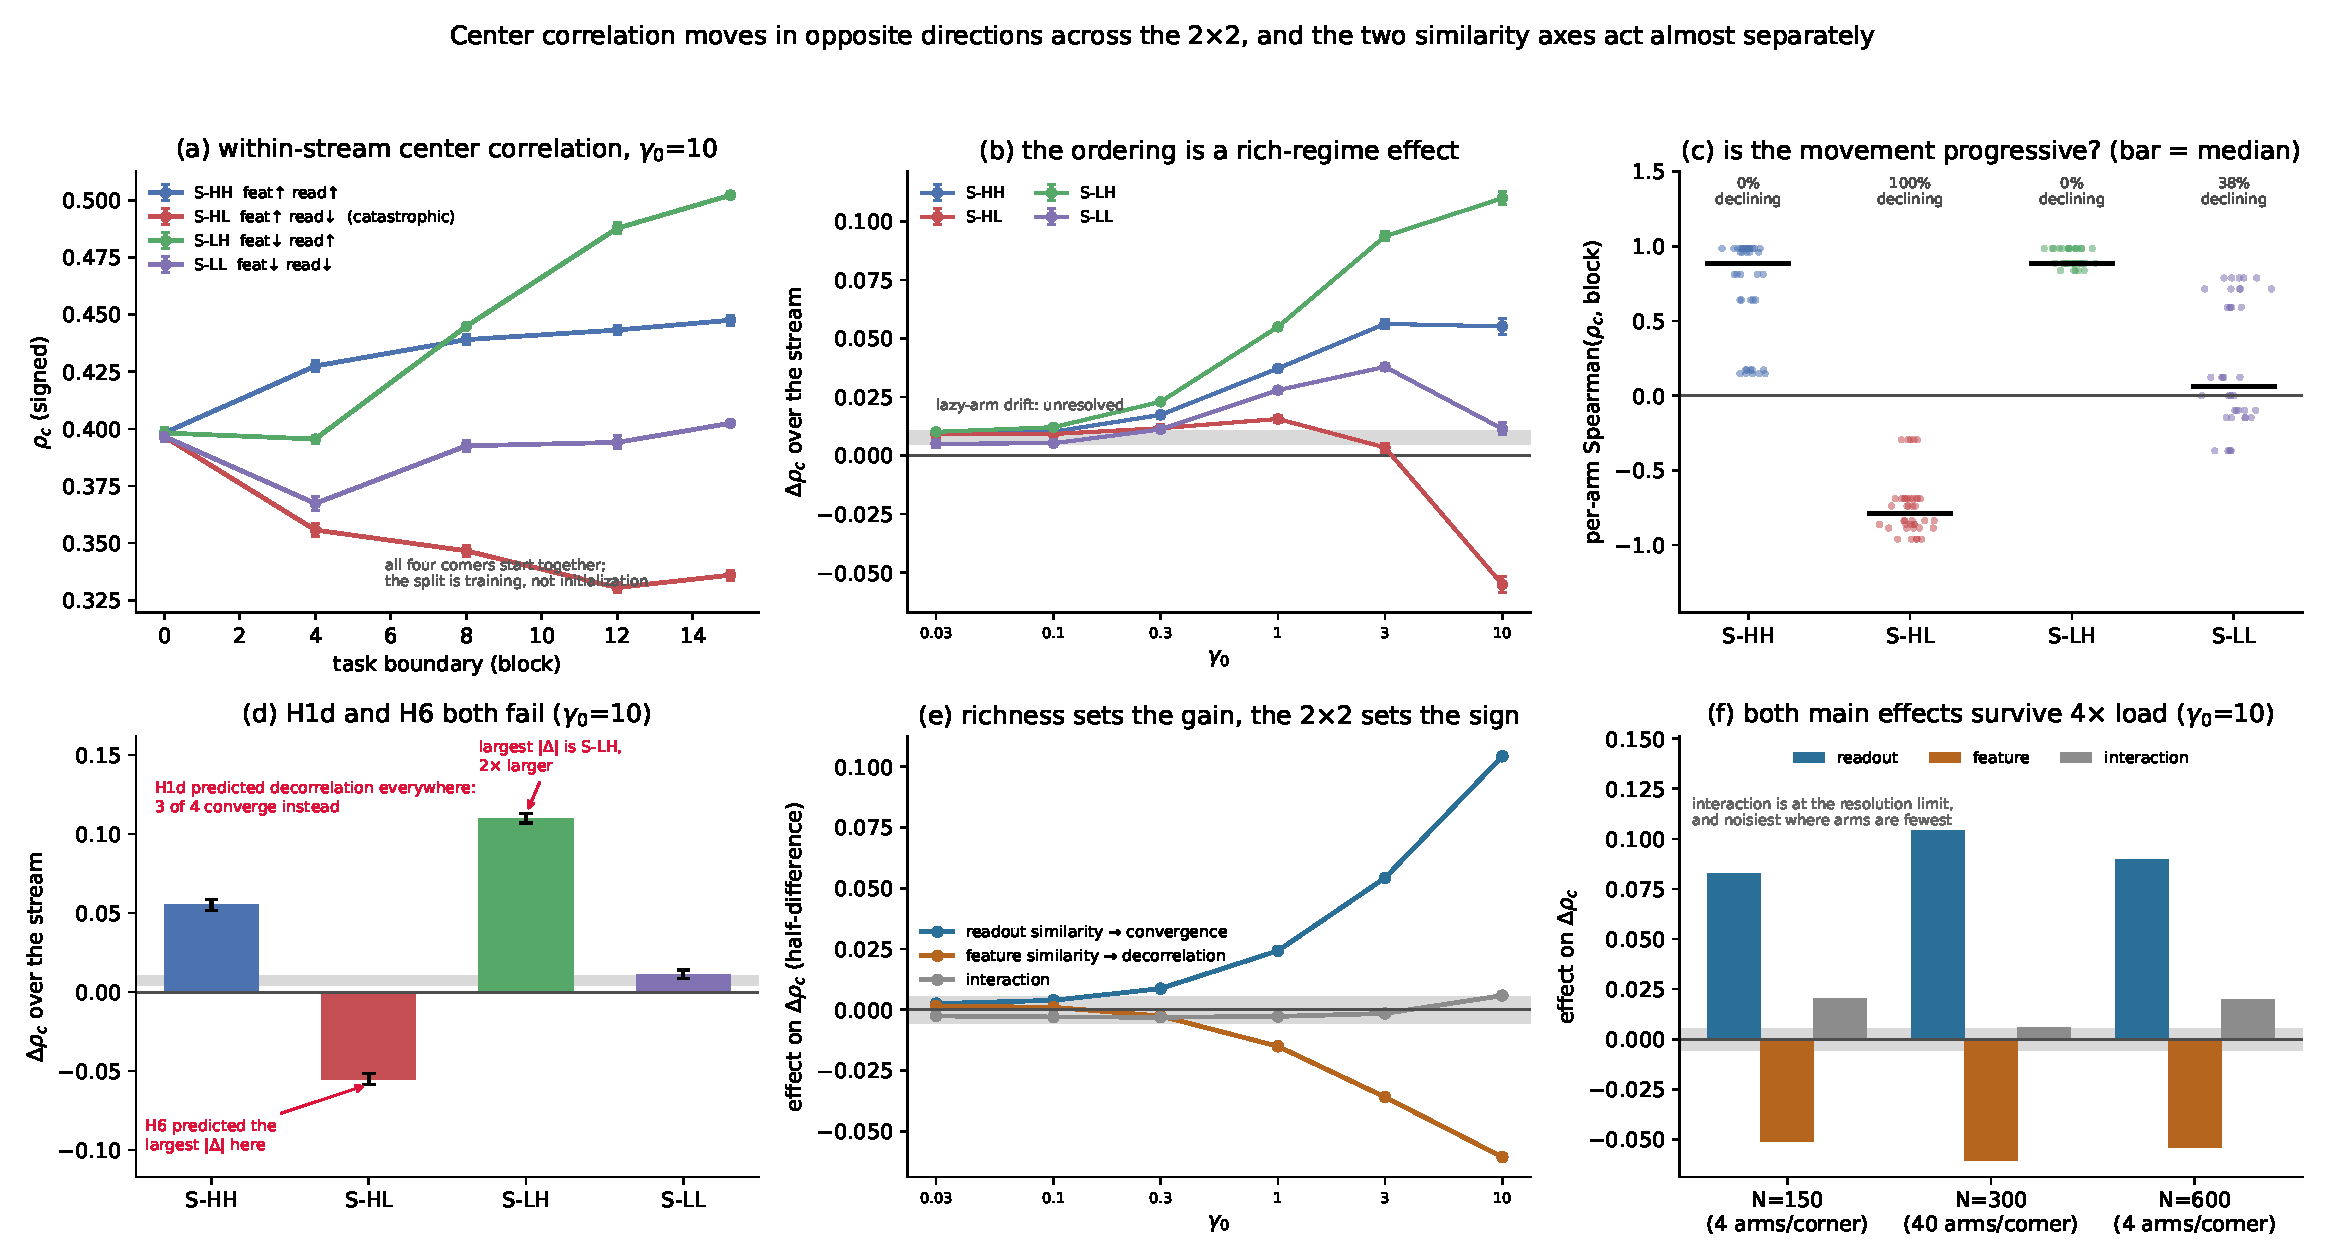
\includegraphics[width=\linewidth]
   {figures/fig4_corners_rho_c__gamma10__960arms__8dd793134c38.pdf}}
\end{figure}
 from the jmlr skeleton's body. Every float uses \floatconts, which the jmlr
% class provides, so captions sit above the graphic and \label lives inside the float.
%
% The \includegraphics filenames are the manifest names verbatim, hashes and arm counts included.
% They are ugly on purpose: the hash is the result set the figure was drawn from and the arm count
% is the n behind it, so a stale PDF cannot be swapped in without the filename changing. Do not
% rename them, and do not strip the hash to tidy the directory listing --- the correspondence to
% figures/MANIFEST.json is what makes the figure checkable, and scripts/check_submission.py
% verifies that every \includegraphics here names a file the manifest currently claims.
%
% Captions are the drafts in docs/07-writeup.md sections D and E, with citations attached.

\begin{figure}[t]
\floatconts
  {fig:decomposition}
  {\caption{\textbf{Forgetting decomposes exactly, and the channel that carries it shifts with
   richness.} Retained capacity for task~0 at lag~12, decomposed by the exact identity of
   \citet{chou2026diagnosing}. Pooled over the three conditions that lose capacity (24 unique seeds
   per $\gamma_0$; 120 files are five copies); \texttt{S-HH} is Figure~\ref{fig:benign}.
   \textbf{(a)}~Magnitude in noise floors, signed: 0.2 at $\gamma_0=0.03$ to 69.7 at $\gamma_0=10$.
   Grey band: $\pm 2$ floors.
   \textbf{(b)}~Channel shares, $|\mathrm{term}|/\sum|\mathrm{term}|$, drawn where the total clears
   the band. $\gamma_0=0.1$ hatched (margin inside the floor's uncertainty); $\gamma_0=0.3$ and
   above solid: utility $0.08\to0.45$, radius $0.39\to0.11$, dimension $0.53\to0.44$ then flat.
   \textbf{(c)}~Signed terms; utility negative on 100\% of arms for $\gamma_0\geq 1$.
   \textbf{(d)}~Center-collapse share of the radius channel, $0.05\to0.44$ through $\gamma_0=3$ then
   flat ($\gamma_0=3\to10$ step unresolved, CI $[-0.038,+0.070]$). Each bar gated at $3\times$ its
   own $R_{\mathrm{eff}}$ floor; coverage is not comparable across bars.
   Lag~12 exists only for task~0, the most-forgotten task --- the largest forgetting in the grid,
   not its average.}}
  {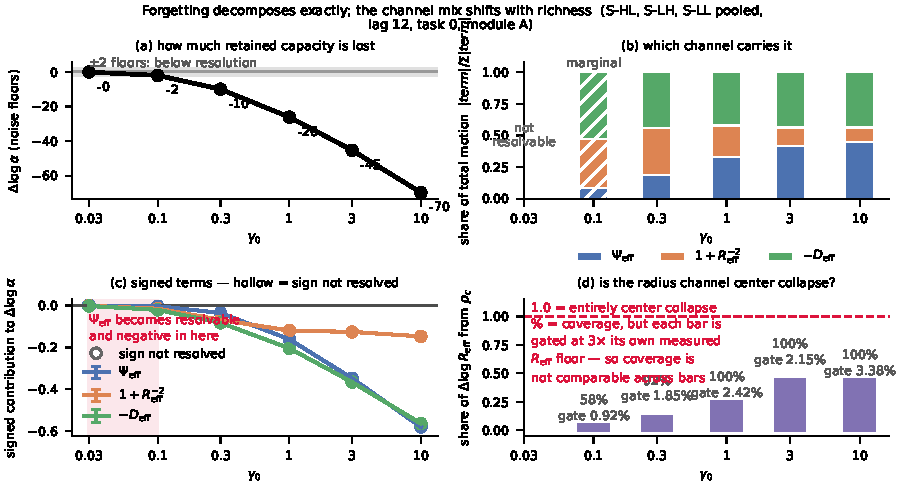
\includegraphics[width=\linewidth]
   {figures/fig2_gamma_sweep__forgetting__lag12__960arms__8dd793134c38.pdf}}
\end{figure}

\begin{figure}[t]
\floatconts
  {fig:corners}
  {\caption{\textbf{Center correlation moves in opposite directions across the similarity design,
   and the two axes act almost separately.}
   \textbf{(a)}~Signed $\rho_c$ at $\gamma_0=10$, design of \citet{hiratani2024disentangling}. All
   four corners start together ($\rho_c = 0.391$--$0.392$); three converge, \texttt{S-HL} (same
   stimuli, different rules) decorrelates.
   \textbf{(b)}~Grey band: lazy-arm drift ($\gamma_0=0.03$). \texttt{S-LL} never leaves it.
   \textbf{(c)}~\texttt{S-HL} decline is progressive, negative on 8 of 8 unique seeds
   ($p=0.0078$, the floor of a two-sided sign test at $n=8$; 40 files are copies), median Spearman
   $-0.79$.
   \textbf{(d)}~H1d and H6 fail in sign: three of four corners converge; largest $|\Delta\rho_c|$ is
   \texttt{S-LH}, twice \texttt{S-HL}.
   \textbf{(e)}~Readout $+0.104$, feature $-0.061$, interaction $+0.006$; additive error $0.012$.
   \textbf{(f)}~Both main effects survive a $4\times$ width change, ordering unchanged.}}
  {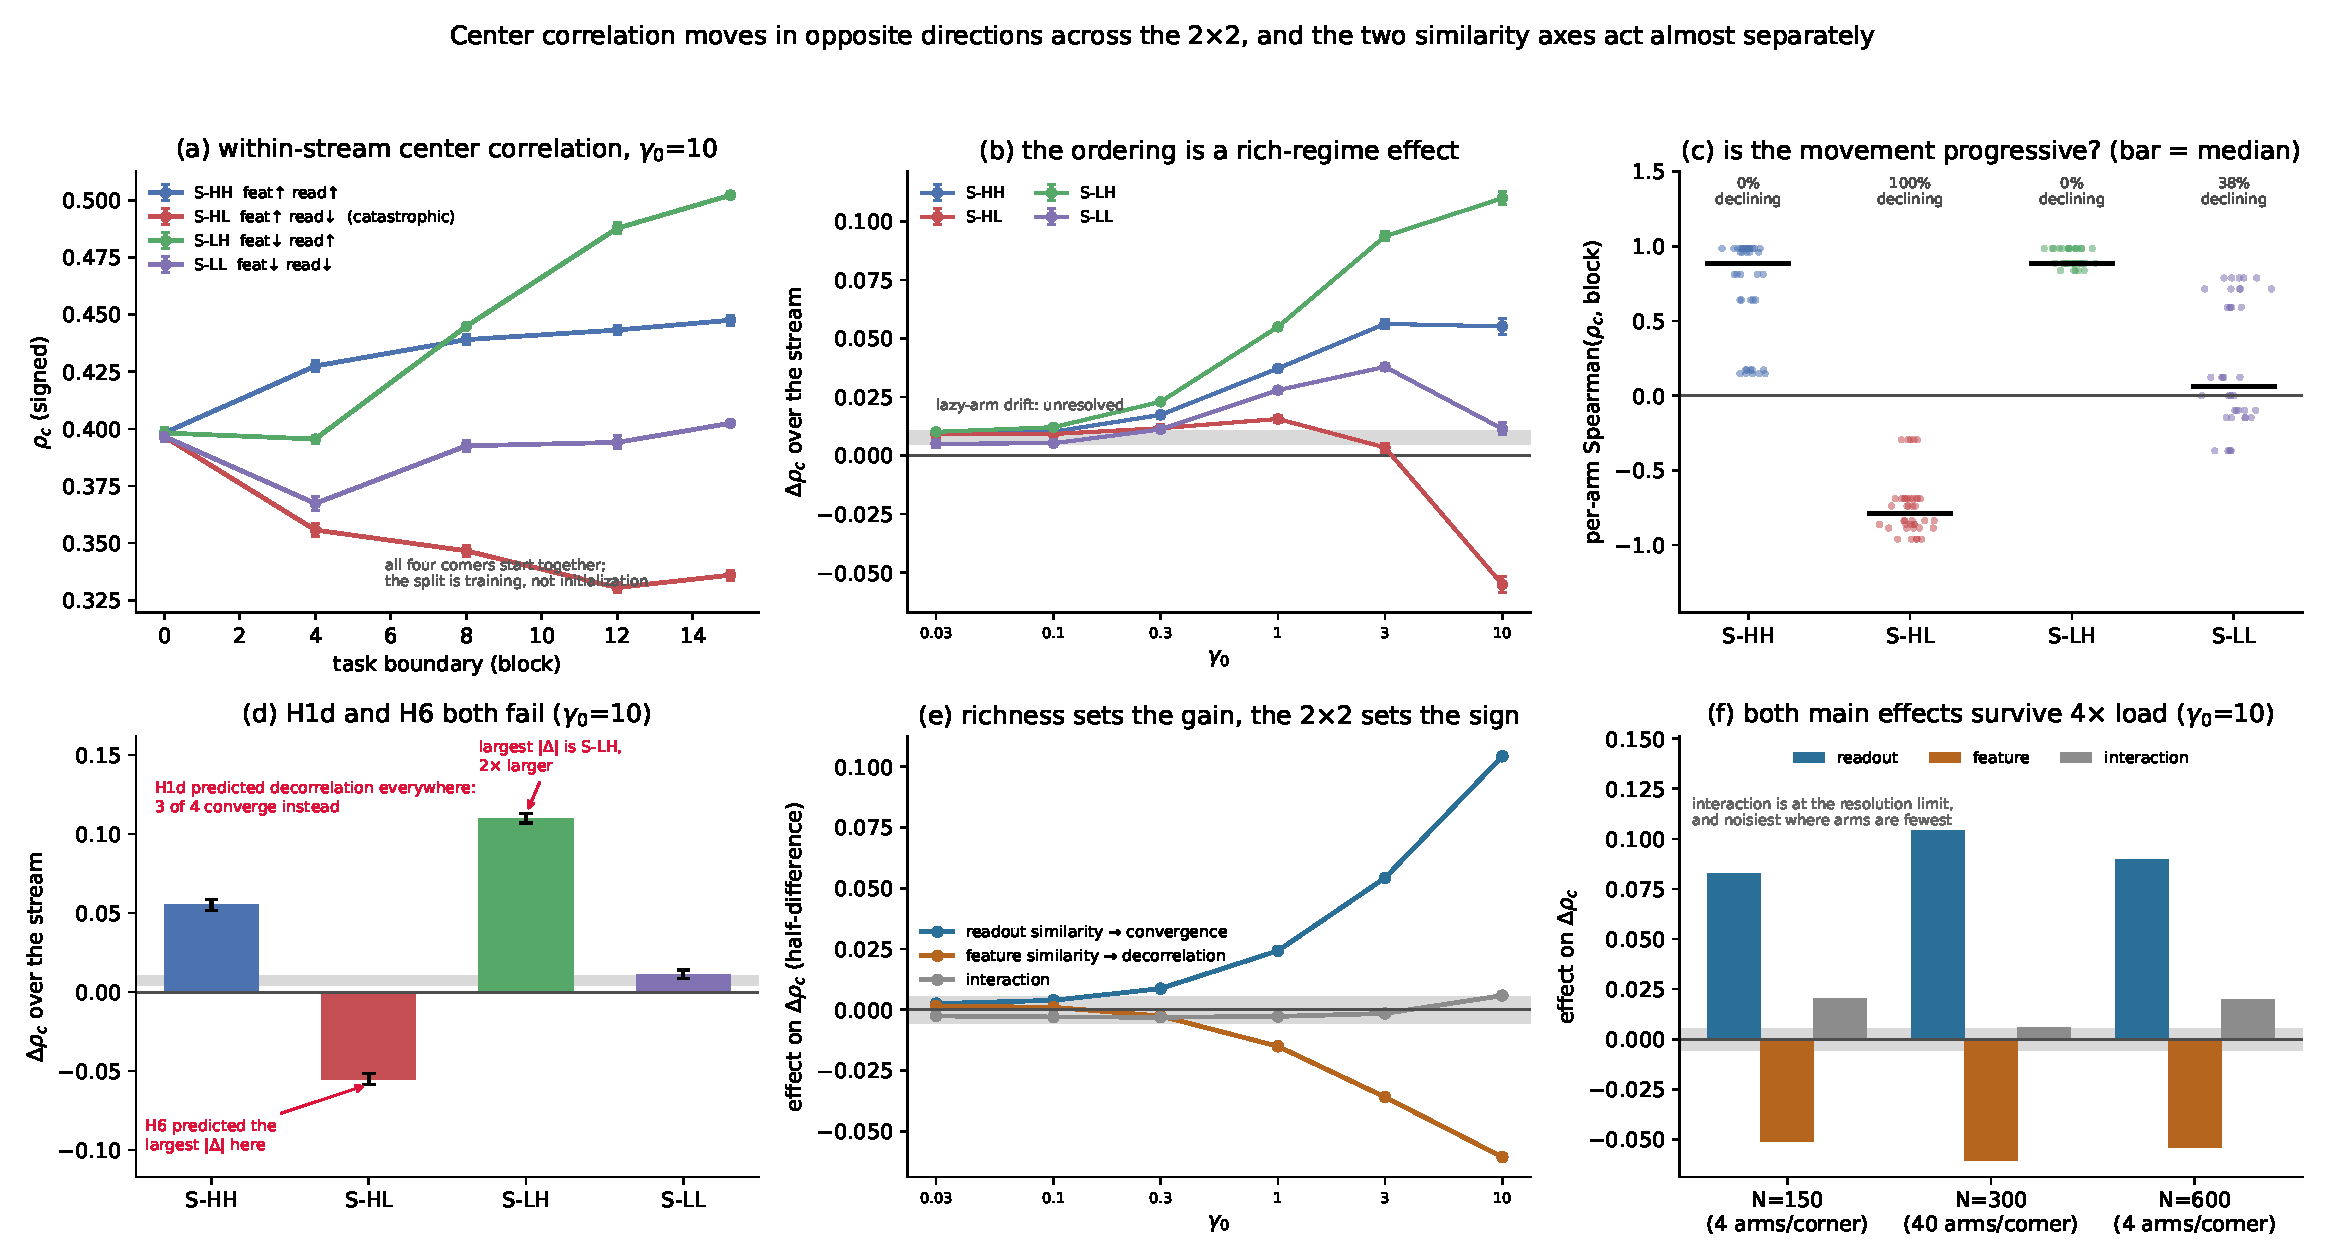
\includegraphics[width=\linewidth]
   {figures/fig4_corners_rho_c__gamma10__960arms__8dd793134c38.pdf}}
\end{figure}
 from the jmlr skeleton's body. Every float uses \floatconts, which the jmlr
% class provides, so captions sit above the graphic and \label lives inside the float.
%
% The \includegraphics filenames are the manifest names verbatim, hashes and arm counts included.
% They are ugly on purpose: the hash is the result set the figure was drawn from and the arm count
% is the n behind it, so a stale PDF cannot be swapped in without the filename changing. Do not
% rename them, and do not strip the hash to tidy the directory listing --- the correspondence to
% figures/MANIFEST.json is what makes the figure checkable, and scripts/check_submission.py
% verifies that every \includegraphics here names a file the manifest currently claims.
%
% Captions are the drafts in docs/07-writeup.md sections D and E, with citations attached.

\begin{figure}[t]
\floatconts
  {fig:decomposition}
  {\caption{\textbf{Forgetting decomposes exactly, and the channel that carries it shifts with
   richness.} Retained capacity for task~0 at lag~12, decomposed by the exact identity of
   \citet{chou2026diagnosing}. Pooled over the three conditions that lose capacity (24 unique seeds
   per $\gamma_0$; 120 files are five copies); \texttt{S-HH} is Figure~\ref{fig:benign}.
   \textbf{(a)}~Magnitude in noise floors, signed: 0.2 at $\gamma_0=0.03$ to 69.7 at $\gamma_0=10$.
   Grey band: $\pm 2$ floors.
   \textbf{(b)}~Channel shares, $|\mathrm{term}|/\sum|\mathrm{term}|$, drawn where the total clears
   the band. $\gamma_0=0.1$ hatched (margin inside the floor's uncertainty); $\gamma_0=0.3$ and
   above solid: utility $0.08\to0.45$, radius $0.39\to0.11$, dimension $0.53\to0.44$ then flat.
   \textbf{(c)}~Signed terms; utility negative on 100\% of arms for $\gamma_0\geq 1$.
   \textbf{(d)}~Center-collapse share of the radius channel, $0.05\to0.44$ through $\gamma_0=3$ then
   flat ($\gamma_0=3\to10$ step unresolved, CI $[-0.038,+0.070]$). Each bar gated at $3\times$ its
   own $R_{\mathrm{eff}}$ floor; coverage is not comparable across bars.
   Lag~12 exists only for task~0, the most-forgotten task --- the largest forgetting in the grid,
   not its average.}}
  {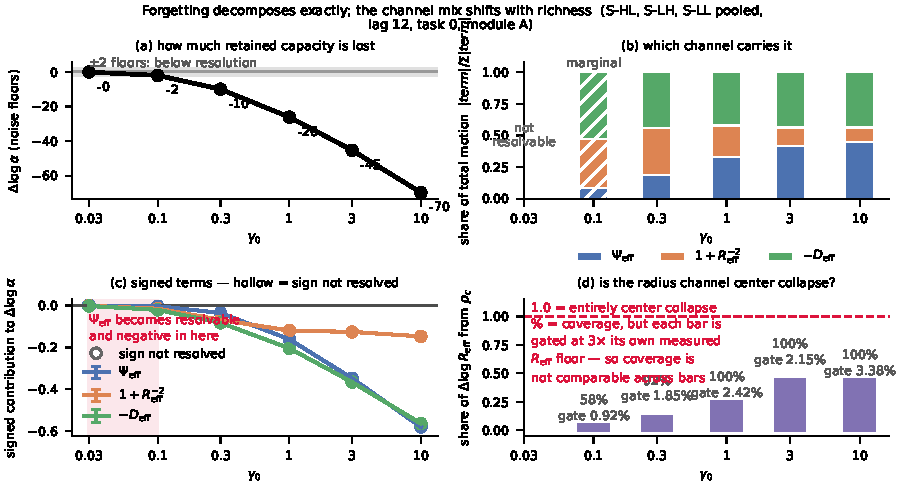
\includegraphics[width=\linewidth]
   {figures/fig2_gamma_sweep__forgetting__lag12__960arms__8dd793134c38.pdf}}
\end{figure}

\begin{figure}[t]
\floatconts
  {fig:corners}
  {\caption{\textbf{Center correlation moves in opposite directions across the similarity design,
   and the two axes act almost separately.}
   \textbf{(a)}~Signed $\rho_c$ at $\gamma_0=10$, design of \citet{hiratani2024disentangling}. All
   four corners start together ($\rho_c = 0.391$--$0.392$); three converge, \texttt{S-HL} (same
   stimuli, different rules) decorrelates.
   \textbf{(b)}~Grey band: lazy-arm drift ($\gamma_0=0.03$). \texttt{S-LL} never leaves it.
   \textbf{(c)}~\texttt{S-HL} decline is progressive, negative on 8 of 8 unique seeds
   ($p=0.0078$, the floor of a two-sided sign test at $n=8$; 40 files are copies), median Spearman
   $-0.79$.
   \textbf{(d)}~H1d and H6 fail in sign: three of four corners converge; largest $|\Delta\rho_c|$ is
   \texttt{S-LH}, twice \texttt{S-HL}.
   \textbf{(e)}~Readout $+0.104$, feature $-0.061$, interaction $+0.006$; additive error $0.012$.
   \textbf{(f)}~Both main effects survive a $4\times$ width change, ordering unchanged.}}
  {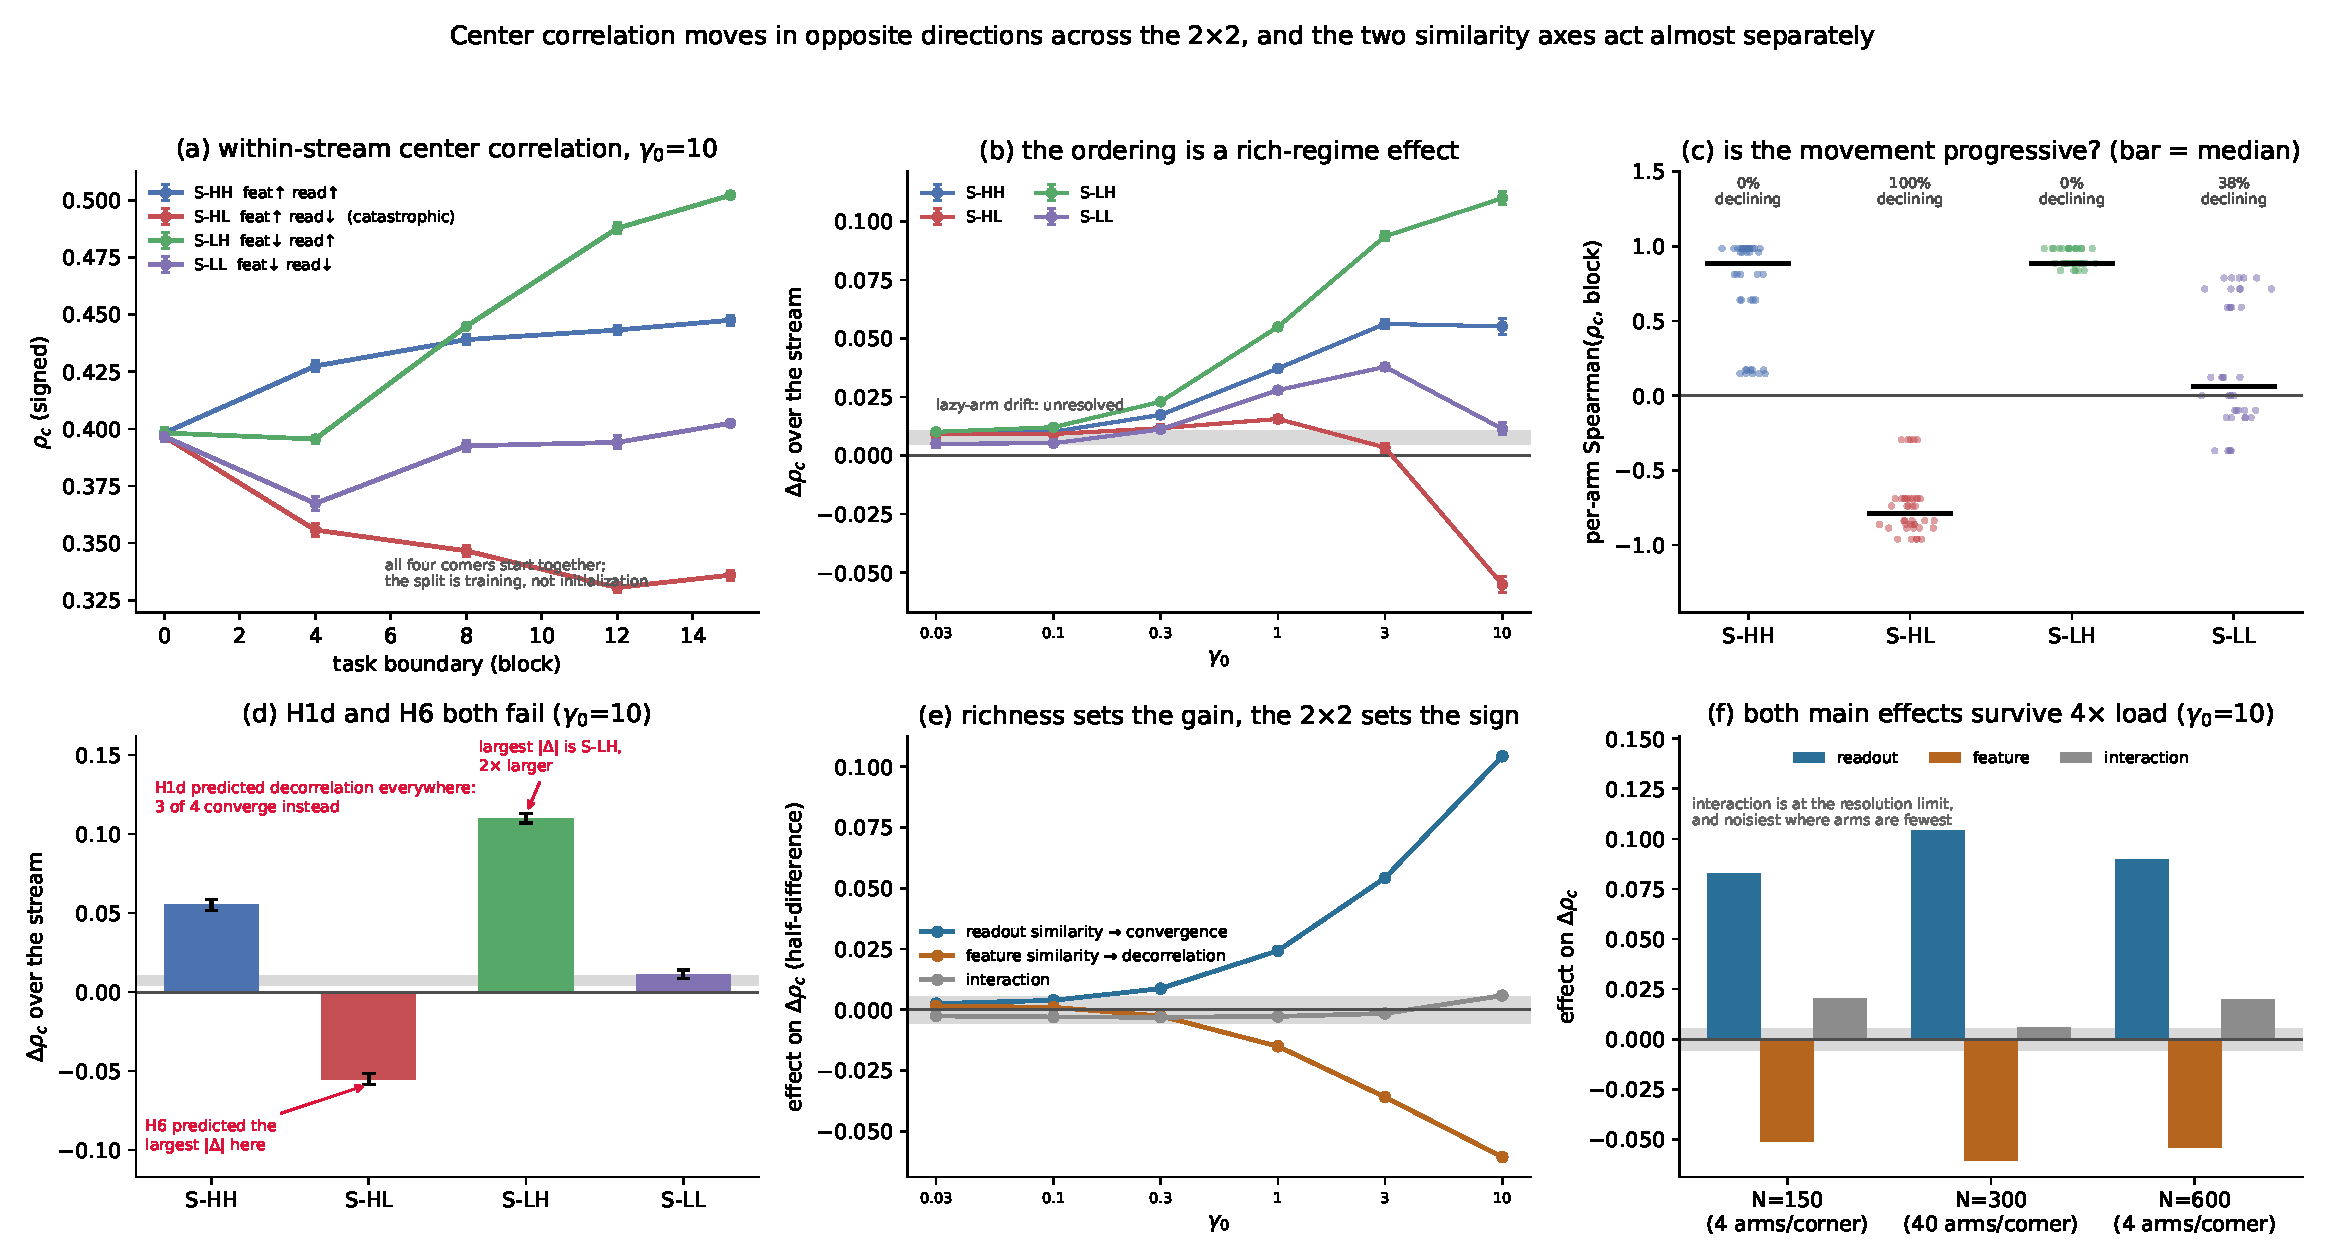
\includegraphics[width=\linewidth]
   {figures/fig4_corners_rho_c__gamma10__960arms__8dd793134c38.pdf}}
\end{figure}

\typeout{HARNESS FIGSEND=\thepage}

\bibliography{../references}
\typeout{HARNESS TOTAL=\thepage}

\end{document}
